%!TEX root = ../bomberchamp.tex

\begin{figure}
  \centering
  % Store largest image in a box
  \savebox{\largestimage}{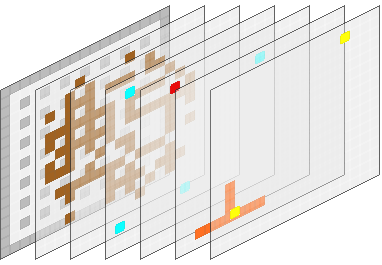
\includegraphics[height=.22\textheight]{images/X_channel-layers.png}}%
  \begin{subfigure}[b]{0.6\textwidth}
    \centering
    \usebox{\largestimage}
    \caption{Visualization of the separate channels}
  \end{subfigure}
  \quad
  \begin{subfigure}[b]{0.36\textwidth}
    \centering
    % Adjust vertical height of smaller image
    \raisebox{\dimexpr.5\ht\largestimage-.5\height}{%
      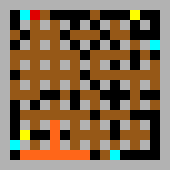
\includegraphics[height=.18\textheight]{images/X_channel-full.png}}
    \caption{All channels combined}
  \end{subfigure}
  \caption{Input channels (from left to right): walls (gray), crates (brown), self (turquoise), other players (turquoise), bombs (red), explosions (orange), coins (yellow)}
  \label{fig:input-channels}
\end{figure}


To simplify learning for our agent, it was centred on the board, so that it stays at a fixed position while the environment (coins, crates, other agents) move around it. To implement this, the size of the board was increased to four times its original size and the agent placed in the middle of the new board.
